\chapter{Results}
\label{results}

\section{Data}
The data set of 250 projects was gathered in July 2013. It contains monthly
data points for each project up to June 2013.

The data set was tested for representativeness using the tool by
\citet{nagappan}. The data set scored a 99.5\% representativeness to the tool's
master data of 20,028 projects tracked by Ohloh.

\paragraph{}
The final data set contains monthly evolution data of 250 distinct projects
having a total of 22,943 data points. The oldest project having 321 monthly
data points, the youngest having 14 monthly data points. The first data point
in the set is of October 1986.

\section{Dead projects}
\label{section:deads}
A total of 38 (15.2\%) projects complied to the definition of a dead project as
defined in section \ref{def:dead}. Manual verification of the 38 potential
dead projects using the project's websites, source code repositories, and
commit history up to April 2014, revealed that 21 (8.4\%) are still complying
to the definition of a dead project in April 2014.

\paragraph{}
The 21 dead projects and their $age\_in\_months$ at the moment of death as a
result of the verification are shown in Table \ref{table:deads}.

\begin{wraptable}{l}{40mm}
\caption{Dead projects}\label{table:deads}
\centering
\begin{tabular}{rr}
  \hline
 ID & Died at month \\ 
  \hline
317799 &   2 \\ 
  587198 &   3 \\ 
  588411 &   5 \\ 
  589515 &   7 \\ 
  587204 &   8 \\ 
  585077 &   9 \\ 
  587571 &  11 \\ 
  586805 &  14 \\ 
  360279 &  30 \\ 
  322065 &  37 \\ 
  11389 &  46 \\ 
  12053 &  68 \\ 
  3085 &  71 \\ 
  307140 &  71 \\ 
  4614 &  75 \\ 
  41745 &  80 \\ 
  155830 &  84 \\ 
  325178 &  92 \\ 
  4007 & 120 \\ 
  15700 & 121 \\ 
  12547 & 142 \\  
   \hline
\end{tabular}
\end{wraptable}

\paragraph{}
All, except one, of the projects in Table \ref{table:deads} are dead because it
was abandoned by the community of contributors. Except for project \#587204,
which is still receiving updates, but at very slow and sporadic intervals.
However, since the updates do not involve code activity, it is considered dead.

\paragraph{}
When looking into project \#317799, which is the youngest in this set and died
in its second month, it shows that this project has had a history of the slightest
change in its lines of code evolution. The project has had a total number of 7
commits during the time it is being tracked by Ohloh (since September 2011). A
total of 4 contributors have worked on the project since it was tracked. The
most recent commit was done in October 2011.

\paragraph{}
Project \#12547 is the oldest. It died after 142 tracked months and has
had its most recent commits in February 2012. A total of 10 contributors have
worked on this project since May 2000.

\paragraph{}
The special case project \#587204, is the only project that is not
abandoned by its (entire) community. The project has had 3 contributors over its
lifetime. One of them is still active every now and then. The most recent
commits were done in January 2014, the commits before that were in June 2012.
The commits involved updates in documentation, and the creation of a
configuration file for a continuous integration server. These commits do not
involve code changes.

The project died in July 2012, after 8 months since the first data point
tracked.

\paragraph{}
From the initial 38 projects, the remaining 17 projects complying to the
definition of dead (section \ref{def:dead}) appeared to be still alive. These
17 projects are evaluated:

\begin{itemize}
	\item For 9 of the projects activity is very low or rapidly decreasing. Their
		community is slowly but surely abandoning the project as can be seen by a
		decrease of 35\% to 55\% of contributors, and/or commits.

	\item 5 of the projects are migrated to another source code repository. For
		these projects the tracking information is not updated at Ohloh and are lost.
		The tracking is stopped from the moment the project is migrated. The tracking
		and analysis can be recovered by updating the source code locations at Ohloh,
		but for this study the project is out of sight.

	\item The 3 projects that have had no activity in a year (i.e, were dead), but
		after that show little increase of activity are more difficult to explain.
		Manual evaluation showed that there exist similar projects outside the data
		set that eventually die, but there are also similar projects that eventually
		got 'resurrected'.
\end{itemize}



\section{Sequences and patterns}
\label{section:seqs_patterns}
The wavelet transform of the LOC signals of 250 projects resulted in 22,943
data points decomposed up to 7 levels into wavelet/shift and filter/scale
coefficients.

\begin{table}[H]
\caption{Similar sequences count}\label{table:sequence_counts}
\centering
\begin{tabular}{lrr}
\hline
	Total & 1,669,448 & 100.000\% \\
	\hline
	In filter/scale coefficients & 1,669,432 & 99.999\% \\
	In wavelet/shift coefficients & 16 & 0.001\% \\
\hline
\end{tabular}
\end{table}


\noindent
As shown in Table \ref{table:sequence_counts}, the similar sequence
identification found a total of 1,669,448 sequences that occurred at least 2
times. A mere 16 sequences were found in wavelet/shift coefficients, the other
1,669,432 sequences were found in filter/scale coefficients.

\paragraph{}
The second wavelet analysis step aggregated similar sequences across multiple
pairs together to form patterns. The detection of these 'popular sequences'
found 16,049 patterns. The patterns consist only of sequences of scale/filter
coefficients.

\paragraph{}
Some patterns that were found are shown in Figure \ref{figure:patterns_plots}.
The four graphs are plots of patterns recomposed onto the original signal,
however, transformed to \textit{relative LOC change} to make them more
comparable in the graph.

The graphs all have multiple ($>$ 140) occurrences of the pattern plotted of one
or more projects in the same graph. The graphs show that the sequences
composing a pattern have similar waveforms. Each graph contains a multiple of
plotted sequences as stated in the figure.

\begin{figure}[H]
\caption{Example of a pattern found during wavelet
analysis}\label{figure:patterns_plots}
\centering
	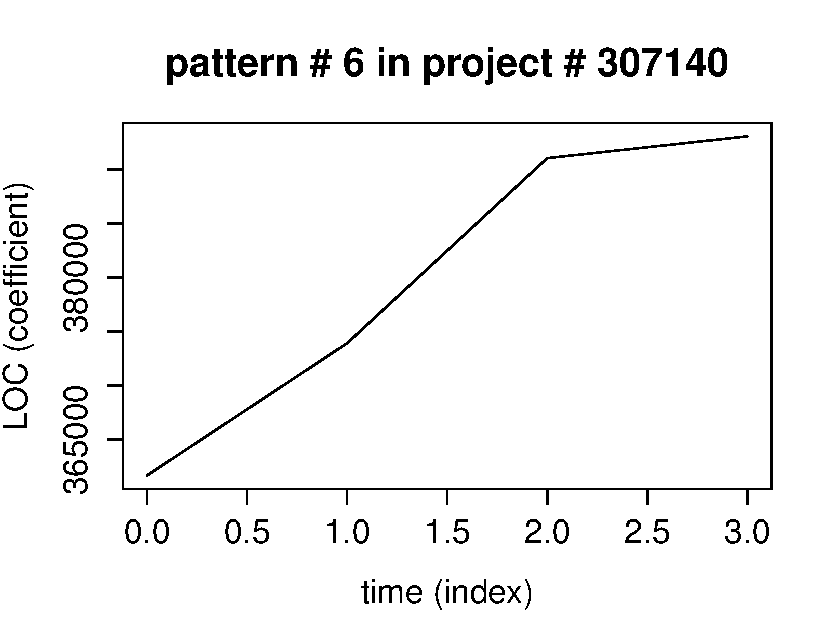
\includegraphics[width=196pt]{images/pattern_6.pdf}\\
	\vspace{1em}
	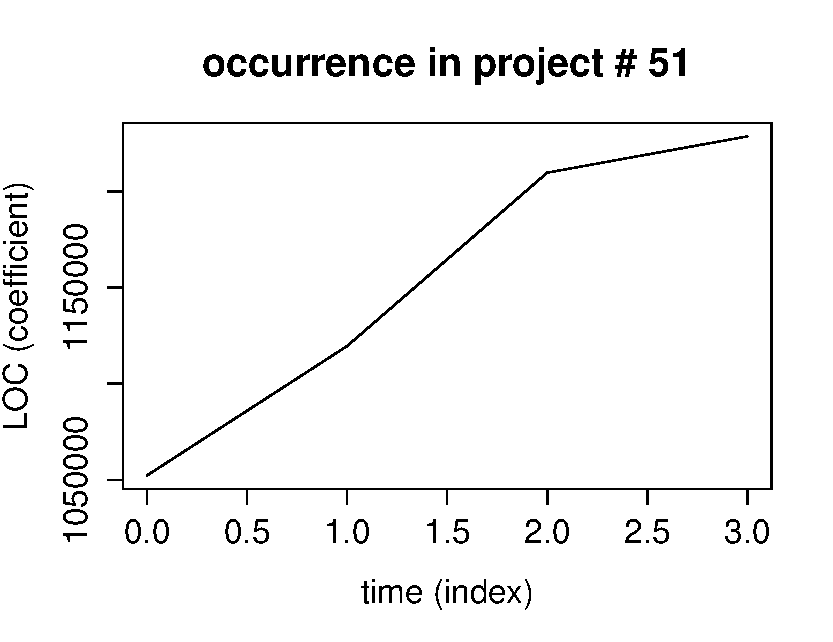
\includegraphics[width=128pt]{images/pattern_6_seq_e.pdf}
	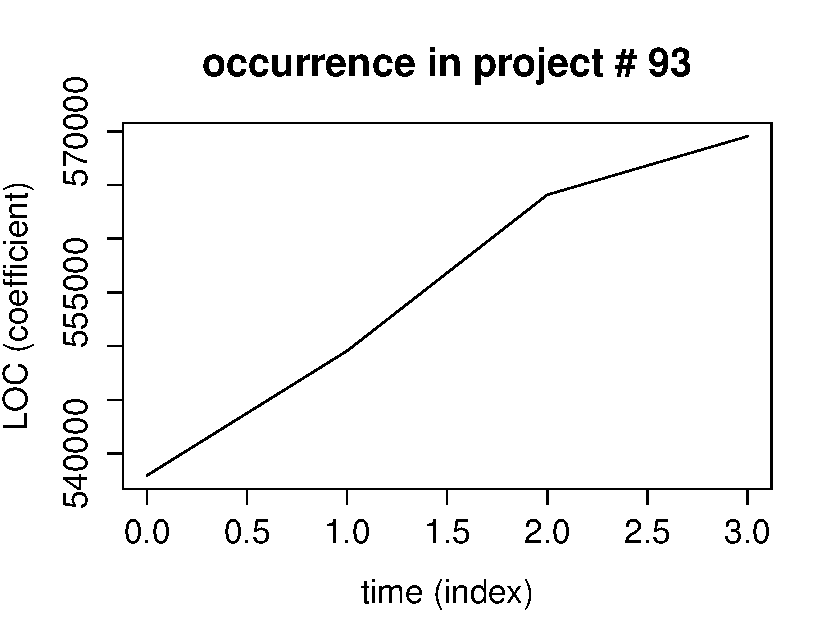
\includegraphics[width=128pt]{images/pattern_6_seq_d.pdf}
	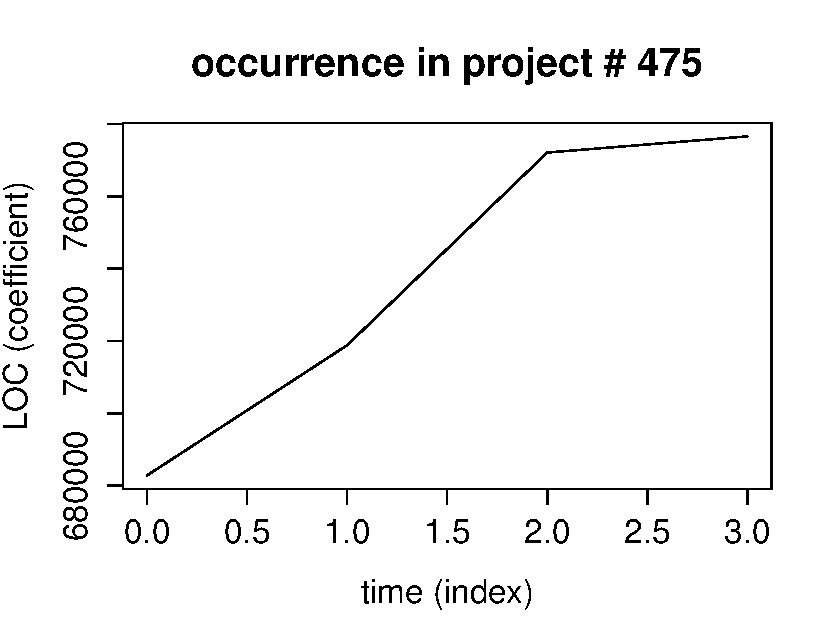
\includegraphics[width=128pt]{images/pattern_6_seq_c.pdf}
	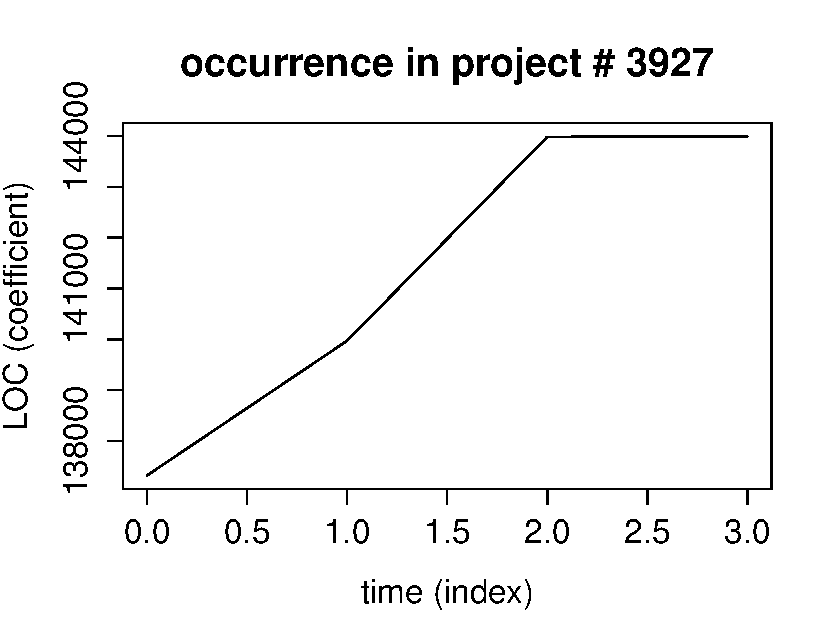
\includegraphics[width=128pt]{images/pattern_6_seq_f.pdf}
	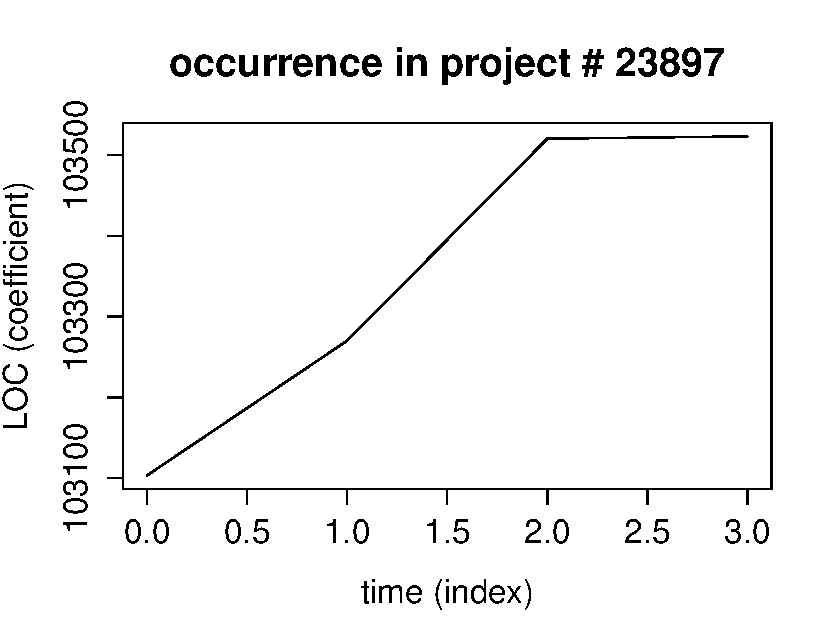
\includegraphics[width=128pt]{images/pattern_6_seq_a.pdf}
	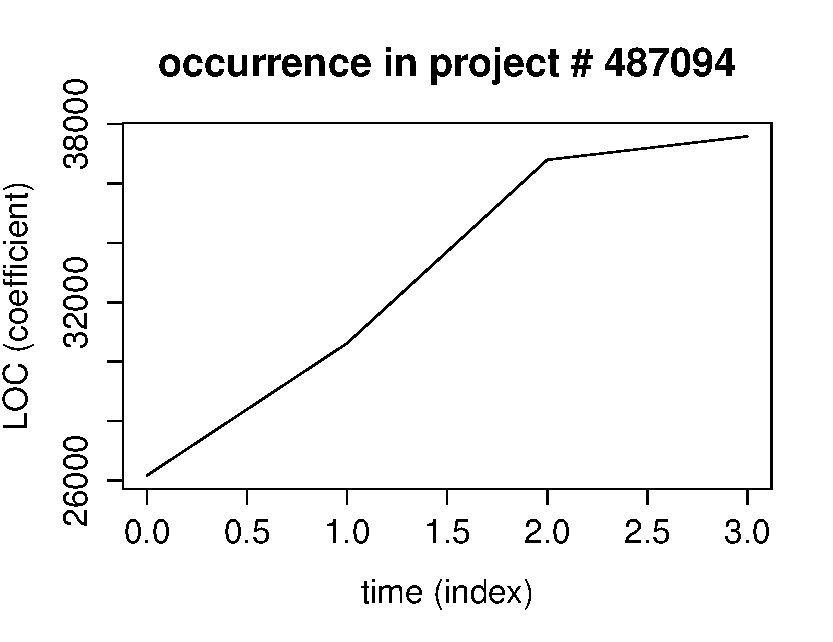
\includegraphics[width=128pt]{images/pattern_6_seq_b.pdf}
\end{figure}

\noindent
Pattern no. 2 illustrates a pattern indicating no change in LOC for 8 months.

\paragraph{}
The patterns occurred between 5 and 1,512 times across the projects. On
average, a pattern occurs 104 times. A single pattern occurs in at least 1 and
at most 204 projects (36 projects on average). The pattern length is between 4
and 19 coefficients (on average 6) across decomposition levels 3 to 7.

On the 3\textsuperscript{th} level, the average pattern length is equal to 4
coefficients. Every subsequent level doubles the average pattern length. This
is expected as there are twice as many coefficients available. This means the
same pattern is detected at multiple levels. Additionally, it can be said that
a pattern has multiple levels.

\paragraph{}
Table \ref{table:pattern_counts} presents the numbers of patterns
detected and occurring across projects. Recall the distinction between
detecting and occurring patterns from section \ref{def:pattern}.

\begin{table}[H]
\caption{Patterns detected and occurring}\label{table:pattern_counts}
\centering
\begin{tabular}{lrr|rr}
\hline
	\bfseries{Patterns detected}\rm & & & \bfseries{Count} \\
	\hline
	total & & & 16,049 & 100.00\% \\
	\hline
	in dead projects & & & 1,084 & 6.75\% \\
	in alive projects & & & 14,965 & 93.25\% \\
\hline\hline
	\bfseries{Patterns detected in dead projects}\rm & \bfseries{Occurrences}\rm
	& & \bfseries{Count}\rm \\
	\hline
	total & 111,848 & 100.00\% & 1,084 & 100.00\% \\
	\hline
	in dead projects only & 111 & 0.10\% & 16 & 1.48\% \\
	%in alive projects only & 0 & 0.00\% & 0 & 0.00\% \\
	in both dead and alive projects & 111,737 & 99.90\% & 1,068 & 98.52\% \\
\hline\hline
	\bfseries{Patterns detected in alive projects}\rm & \bfseries{Occurrences}\rm & & \bfseries{Count}\rm \\
	\hline
	total & 1,560,883 & 100.00\% & 14,965 & 100.00\% \\
	\hline
	%in dead projects only & 0 & 0.00\% & 0 & 0.00\% \\
	in alive projects only & 37,333 & 2.39\% & 3,390 & 22.65\% \\
	in both dead and alive projects & 1,523,550 & 97.61\% & 11,575 & 77.35\% \\
\hline
\end{tabular}
\end{table}

\noindent
As can be seen from Table \ref{table:pattern_counts}, 16,049 patterns were
detected across 250 projects, which is 64.2 patterns per project on average;
14,965 patterns were detected across 229 alive projects (65.3 patterns on
average per project); and 1,084 patterns detected in 21 dead projects (an
average of 51.6 patterns per project). The averages do not differ significantly
over the projects.



\section{Pattern classification}
The classification of the patterns was done to distinguish different types of
patterns to be able to find evolutionary events. For this, the patterns
detected in dead projects were taken and classified according to
the definitions in section \ref{section:patterns_dead}. It is expected that
this group has the highest chance of keeping a pattern indicating an
evolutionary event leading to the end of code evolution.

\paragraph{}
A total of 1,084 patterns detected in dead projects is classified. The sizes of
the pattern type subsets are shown in Table \ref{table:pattern_type_counts}.
For each subset, it is stated in how many projects a pattern of that type was
found.

\begin{table}[H]
\caption{Pattern types}\label{table:pattern_type_counts}
\centering
\begin{tabular}{rrr|rr}
\hline
	\bfseries{Type}\rm & \bfseries{Pattern count}\rm & & \bfseries{Occurrences}\rm
	& \bfseries{Project count}\rm \\
	\hline
	A & 13 & 1.20\% & 167 & 93 \\
	B & 382 & 35.24\% & 10,741 & 204 \\
	AB & 689 & 63.56\% & 100,967 & 226 \\
	\hline
	 & 1,084 & 100.00\% &  \\
\hline
\end{tabular}
\end{table}


\noindent
The patterns of all three groups were detected in dead projects, but may occur
in both dead and alive projects.

In search of patterns that lead to the end of code evolution, patterns of type
A will be most interesting, because these patterns last until the end of
evolution data of dead projects.

The evaluation of type A patterns is described in section
\ref{section:kp_survival}.

\begin{comment}
- Factual results
- Tables and figures for clarification

This chapter presents and clarifies the results obtained during the research.
The focus should be on the factual results, not the interpretation or
discussion. Tables and graphics should be used to increase the clarity of the
results where applicable.
Have a look at the the results chapter in this example thesis on Paul’s
homepage\footnote{http://homepages.cwi.nl/~paulk/thesesMasterSoftwareEngineering/2006/ArnoldLankamp.pdf}.
\end{comment}
